% Knowledge Pipeline — Concept Diagram
% Compile with: pdflatex knowledge-pipeline.tex
\documentclass[border=12pt]{standalone}

\usepackage[T1]{fontenc}
\usepackage[english]{babel}
\usepackage{lmodern}
\usepackage{amsmath}
\usepackage{xcolor}
\usepackage{tikz}
\usetikzlibrary{
    decorations.pathmorphing,
    decorations.pathreplacing,
    arrows.meta,
    positioning,
    calc,
    shapes.geometric,
    backgrounds,
    fadings
}

%% ---------- Colour palette ----------
\definecolor{ink}      {HTML}{1F2433}  % near-black outlines / text
\definecolor{think}    {HTML}{4A6FA5}  % cool blue — "Denken"
\definecolor{thinkbg}  {HTML}{E8EEF7}
\definecolor{lens}     {HTML}{C8553D}  % warm red — "Linse / Agenten"
\definecolor{lensbg}   {HTML}{FBEBE6}
\definecolor{coil}     {HTML}{6B7280}
\definecolor{node}     {HTML}{2E3A59}
\definecolor{nodebg}   {HTML}{F2F4F8}
\definecolor{accent}   {HTML}{3A6E5B}  % muted green for distillate flow
\definecolor{soft}     {HTML}{8A93A6}

\begin{document}
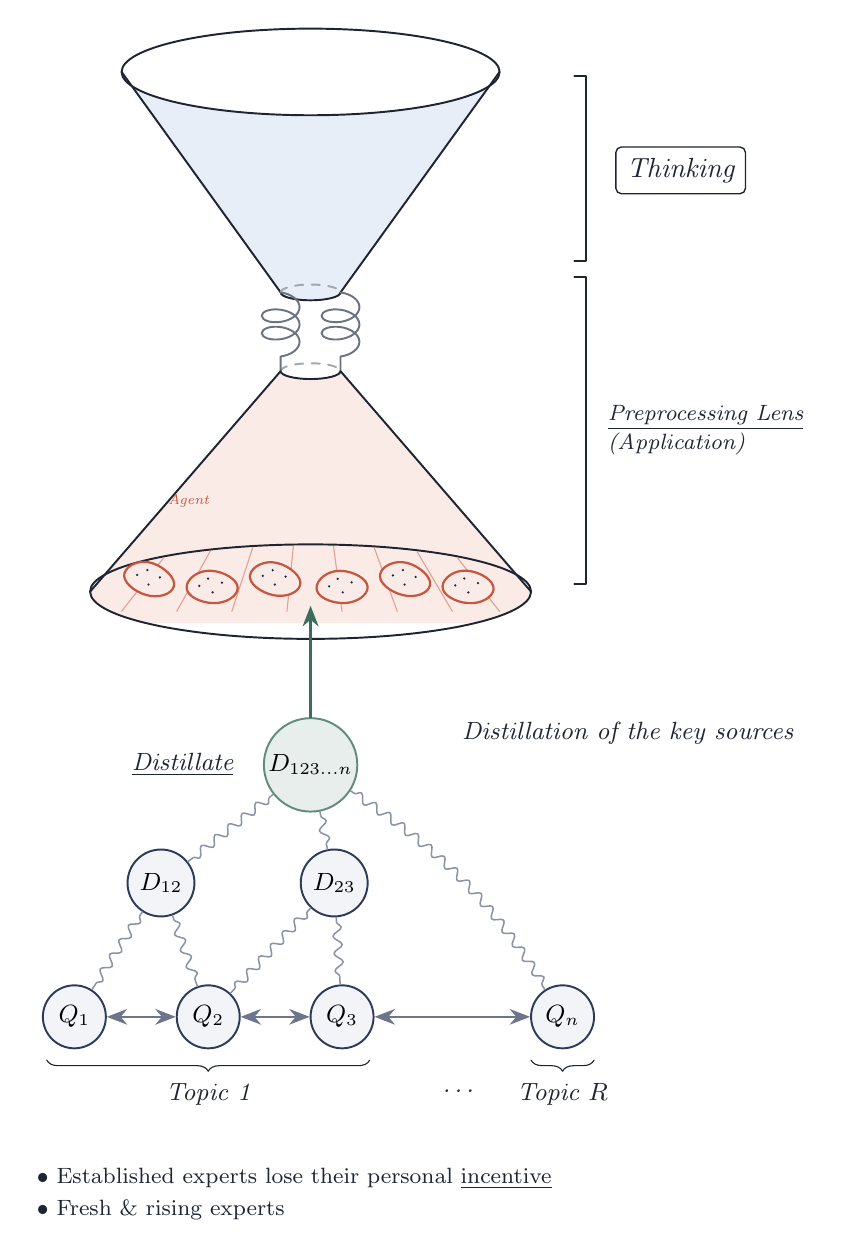
\begin{tikzpicture}[
    line cap=round, line join=round,
    >={Stealth[length=2.6mm, width=2.0mm]},
    %% --- semantic styles ---
    outline/.style   = {draw=ink, line width=0.7pt},
    coilline/.style  = {draw=coil, line width=0.7pt},
    agent/.style     = {draw=lens, line width=0.8pt, fill=lens!12},
    dnode/.style     = {circle, draw=node, line width=0.7pt,
                        fill=nodebg, minimum size=8.5mm,
                        inner sep=1pt, font=\small},
    dlabel/.style    = {font=\itshape\small, text=ink},
    sectionlabel/.style = {font=\itshape, text=ink,
                           draw=ink, line width=0.5pt,
                           rounded corners=2pt,
                           inner sep=4pt, fill=white},
    squiggly/.style  = {draw=soft, line width=0.55pt,
                        decorate, decoration={snake,
                            amplitude=0.55mm, segment length=2.2mm,
                            post length=0.6mm, pre length=0.6mm}},
    flow/.style      = {->, draw=accent, line width=1.1pt},
    sideArrow/.style = {<->, draw=node!70, line width=0.55pt},
    note/.style      = {font=\footnotesize, text=ink, align=left}
]

%% ============================================================
%% HOURGLASS — top funnel (Denken) + coil + bottom funnel (Linse)
%% ============================================================

%% key coordinates
\coordinate (Otop)  at (0, 7.0);   % centre of top opening
\coordinate (Wtop)  at (0, 4.2);   % top of waist
\coordinate (Wbot)  at (0, 3.2);   % bottom of waist
\coordinate (Obot)  at (0, 0.4);   % centre of bottom opening

\def\Rtop{2.4}     % radius of top opening
\def\Ywall{0.55}   % vertical squash for ellipses
\def\Rwaist{0.38}  % radius at the waist
\def\Ywaist{0.10}
\def\Rbot{2.8}     % radius of bottom opening
\def\Ybot{0.60}

%% --- soft fill for the top half (Denken) ---
\begin{scope}
  \clip
    ($(Otop)+(-\Rtop,0)$)
      arc[start angle=180, end angle=360, x radius=\Rtop, y radius=\Ywall]
      -- ($(Wtop)+(\Rwaist,0)$)
      arc[start angle=0,   end angle=-180, x radius=\Rwaist, y radius=\Ywaist]
      -- cycle;
  \fill[thinkbg] (-3,3) rectangle (3,7.6);
\end{scope}

%% --- soft fill for the bottom half (Linse) ---
\begin{scope}
  \clip
    ($(Wbot)+(-\Rwaist,0)$)
      arc[start angle=180, end angle=360, x radius=\Rwaist, y radius=\Ywaist]
      -- ($(Obot)+(\Rbot,0)$)
      arc[start angle=0,   end angle=-180, x radius=\Rbot, y radius=\Ybot]
      -- cycle;
  \fill[lensbg] (-3.2,0) rectangle (3.2,3.4);
\end{scope}

%% --- TOP funnel outline ---
% top opening (ellipse, front + back)
\draw[outline] (Otop) ellipse [x radius=\Rtop, y radius=\Ywall];
% side walls
\draw[outline] ($(Otop)+(-\Rtop,0)$) -- ($(Wtop)+(-\Rwaist,0)$);
\draw[outline] ($(Otop)+( \Rtop,0)$) -- ($(Wtop)+( \Rwaist,0)$);

%% --- Waist coil (the "filter") ---
% top + bottom rims of the coil section
\draw[outline] ($(Wtop)+(-\Rwaist,0)$)
    arc[start angle=180, end angle=360, x radius=\Rwaist, y radius=\Ywaist];
\draw[outline, dashed, draw=ink!40]
    ($(Wtop)+(-\Rwaist,0)$)
    arc[start angle=180, end angle=0, x radius=\Rwaist, y radius=\Ywaist];
\draw[outline] ($(Wbot)+(-\Rwaist,0)$)
    arc[start angle=180, end angle=360, x radius=\Rwaist, y radius=\Ywaist];
\draw[outline, dashed, draw=ink!40]
    ($(Wbot)+(-\Rwaist,0)$)
    arc[start angle=180, end angle=0, x radius=\Rwaist, y radius=\Ywaist];
% the coil itself (two vertical springs on either side)
\draw[coilline,
      decorate, decoration={coil, aspect=0.55,
                            segment length=2.2mm, amplitude=2.4mm}]
    ($(Wtop)+(-\Rwaist,0)$) -- ($(Wbot)+(-\Rwaist,0)$);
\draw[coilline,
      decorate, decoration={coil, aspect=0.55,
                            segment length=2.2mm, amplitude=2.4mm}]
    ($(Wtop)+( \Rwaist,0)$) -- ($(Wbot)+( \Rwaist,0)$);

%% --- BOTTOM funnel outline ---
\draw[outline] ($(Wbot)+(-\Rwaist,0)$) -- ($(Obot)+(-\Rbot,0)$);
\draw[outline] ($(Wbot)+( \Rwaist,0)$) -- ($(Obot)+( \Rbot,0)$);
% bottom ellipse
\draw[outline] (Obot) ellipse [x radius=\Rbot, y radius=\Ybot];

%% --- Agent fan-lines + agent clusters inside the lens ---
\begin{scope}
  % clip to the bottom dish so nothing leaks outside
  \clip (Obot) ellipse [x radius=\Rbot-0.02, y radius=\Ybot-0.02];
  % red light-rays radiating from the waist into the lens
  \foreach \x in {-2.4,-1.7,-1.0,-0.3,0.4,1.1,1.8,2.4} {
    \draw[lens!55, line width=0.4pt] (0,3.2) -- (\x,0.15);
  }
\end{scope}

% Agent clusters (small "amoebas" of data points) along the dish floor
\foreach \cx/\cy/\rot in {
    -2.05/0.55/-8, -1.25/0.45/6, -0.45/0.55/-4,
     0.40/0.45/8,   1.20/0.55/-6,  2.00/0.45/4}
{
  \begin{scope}[shift={(\cx,\cy)}, rotate=\rot]
    \draw[agent] plot[smooth cycle, tension=0.9]
        coordinates {(-0.32,0) (-0.05,0.22) (0.32,0) (0.05,-0.20)};
    \foreach \dx/\dy in {-0.16/0.04, 0/-0.06, 0.13/0.05, -0.04/0.12} {
        \fill[ink] (\dx,\dy) circle (0.45pt);
    }
  \end{scope}
}
% small "Agent" label in red, like the original
\node[font=\tiny\itshape, text=lens] at (-1.55, 1.55) {Agent};

%% ============================================================
%% RIGHT-SIDE BRACKETS + SECTION LABELS
%% ============================================================
\def\BX{3.35} % bracket x-position

% Thinking bracket (top half)
\draw[outline] (\BX,6.95) -- ++(0.15,0) -- ($(\BX+0.15, 4.6)$) -- ++(-0.15,0);
\node[sectionlabel] at (\BX+1.35, 5.75) {Thinking};

% Preprocessing Lens bracket (bottom half)
\draw[outline] (\BX,4.4) -- ++(0.15,0) -- ($(\BX+0.15, 0.5)$) -- ++(-0.15,0);
\node[note, anchor=west] at (\BX+0.30, 2.45)
    {\itshape\underline{Preprocessing Lens}\\[1pt]\itshape (Application)};

%% ============================================================
%% DISTILLATE → SOURCES TREE  (below the hourglass)
%% ============================================================

% Root (Destillat)
\node[dnode, fill=accent!12, draw=accent!80] (Droot)
    at (0, -1.8) {$D_{123\dots n}$};
\node[dlabel, anchor=east] at ($(Droot.west)+(-0.25,0)$)
    {\underline{Distillate}};
\node[dlabel, anchor=west] at (1.8, -1.4)
    {Distillation of the key sources};

% Intermediate distillates
\node[dnode] (D12) at (-1.9, -3.3) {$D_{12}$};
\node[dnode] (D23) at ( 0.3, -3.3) {$D_{23}$};

% Sources Q1..Qn
\node[dnode, minimum size=8mm] (Q1) at (-3.0, -5.0) {$Q_1$};
\node[dnode, minimum size=8mm] (Q2) at (-1.3, -5.0) {$Q_2$};
\node[dnode, minimum size=8mm] (Q3) at ( 0.4, -5.0) {$Q_3$};
\node[dnode, minimum size=8mm] (Qn) at ( 3.2, -5.0) {$Q_n$};

% Distillation links (squiggly = "informal aggregation")
\draw[squiggly] (Droot) -- (D12);
\draw[squiggly] (Droot) -- (D23);
\draw[squiggly] (Droot) to[bend left=12] (Qn);

\draw[squiggly] (D12) -- (Q1);
\draw[squiggly] (D12) -- (Q2);
\draw[squiggly] (D23) -- (Q2);
\draw[squiggly] (D23) -- (Q3);

% Lateral discussion arrows between sources
\draw[sideArrow] (Q1) -- (Q2);
\draw[sideArrow] (Q2) -- (Q3);
\draw[sideArrow] (Q3) -- (Qn);

% Themes (Themen) under the sources
\draw[decorate, decoration={brace, mirror, amplitude=4pt}, draw=ink]
    (-3.35,-5.55) -- (0.75,-5.55)
    node[midway, below=5pt, dlabel] {Topic 1};
\node[dlabel] at (1.9,-5.95) {\ldots};
\draw[decorate, decoration={brace, mirror, amplitude=4pt}, draw=ink]
    (2.8,-5.55) -- (3.6,-5.55)
    node[midway, below=5pt, dlabel] {Topic $R$};

%% --- Flow arrow: distillate → bottom of the lens ---
\draw[flow] (Droot.north) -- ($(Obot)+(0,-0.18)$);

%% ============================================================
%% NOTES UNDER THE DIAGRAM
%% ============================================================
\node[note, anchor=north west] at (-3.6, -6.8)
    {$\bullet$~Established experts lose their
       personal \underline{incentive}\\[2pt]
     $\bullet$~Fresh \& rising experts};

\end{tikzpicture}
\end{document}
